\documentclass[11pt,a4paper]{article}
\usepackage[T1]{fontenc}
\usepackage{lmodern,microtype,amsmath,amssymb,booktabs,tabularx}
\usepackage[margin=27mm]{geometry}
\usepackage[dvipsnames]{xcolor}
\usepackage[colorlinks=true,linkcolor=MidnightBlue,urlcolor=MidnightBlue]{hyperref}
\usepackage{pdfpages}
\setlength{\emergencystretch}{2em}
\hypersetup{pdftitle={Four research advances from the ProveIt GRH analysis},pdfauthor={Research notes prepared for Vladimir Reshetnikov}}
\title{\textbf{Four research advances from the ProveIt GRH analysis}\\[8pt]\large Sharp positive filters, optimal subfield detectors,\\ sparse $p$-adic roots, and quadratic rigidity}
\author{Research notes prepared for Vladimir Reshetnikov}
\date{27 November 2026}
\begin{document}
\maketitle

\section*{Outcome and reading guide}
This collection gives four complete research arguments developed from the mechanisms and open questions in the supplied repository. The main theorems are unconditional. Interpreting the first theorem as cancellation of every nonzero \emph{real} zero ordinate uses the repository's stated Dirichlet-GRH input. No proof of a prominent general conjecture, including nonabelian GRH or Artin holomorphy, is claimed.

The work is based on the immutable ProveIt snapshot
\begin{center}\small\texttt{ce35f320bc88c02093e479f5fe5003ff86b2795f}.\end{center}
The article's quoted upstream Lean theorem has scope RH and Dirichlet GRH over $\mathbb Q$; the present work does not repeat its build or kernel replay. Newness is assessed relative to the pinned article, relevant incoming reports, and targeted literature searches. It is not a certification of worldwide priority. The proofs were cross-reviewed within this research session; they have not undergone external peer review or Lean formalization.

\begin{center}\small
\begin{tabularx}{\textwidth}{@{}lX@{}}\toprule
Note & Main advance\\\midrule
1. Endpoint filters & Necessary double-exponential coefficient improves from $2\pi d/Q_*$ to $\pi d/Q_*$; exact zeta--beta attainment range.\\
2. Subfield detectors & Optimal maximum degree for $\mathrm{PSL}_2(q)$ when $q\equiv1\pmod4$, with exception $q=9$; unconditional zero detection.\\
3. Sparse roots & Exact values at $2p+2$, $2p+3$, and $2p+4$ monomials; the last threshold jumps to $p^2+p$.\\
4. Filter rigidity & General variance formula for the width Hessian and its exact reflection-symmetry kernel.\\\bottomrule
\end{tabularx}
\end{center}

Each note includes its definitions, proofs, source comparison, limitations, and references. The archive also includes every \LaTeX{} source, standalone PDFs, verification scripts and their output, a source audit, a build script, and checksums. The computations check finite algebra and examples; the uniform mathematical proofs are in the manuscripts.

\clearpage
\section*{1. A sharp uncertainty principle for positive zero filters}
Let a finite conjugation-closed multiset of primitive Dirichlet characters have total degree $d$ and geometric mean conductor $Q_*$. Include the conductor-one zeta completion if desired. Divide the product of the completions by its central zero and call the resulting even entire function of the Fourier variable $\Psi$.

If a probability measure $\mu$ has entire Fourier transform $F_\mu$ with $F_\mu/\Psi$ entire, then
\[
 \int_{\mathbb R}\exp\!\bigl(b e^{2|t|/d}\bigr)\,d\mu(t)<\infty
 \quad\Longrightarrow\quad b\le\frac{\pi d}{Q_*}.
\]
The bound is strict if $A=\frac12\sum a_\chi-\frac d4+2r-m\ge0$, where $a_\chi$ is parity, $r$ counts zeta factors, and $m$ is the product's central multiplicity. For $r$ zeta factors and $s$ beta factors, the exact feasible range is
\[
 0<b<\frac{\pi(r+s)}{4^{s/(r+s)}}.
\]
An explicit positive theta convolution works for every coefficient in this interval. The proof uses the directional indicator of the entire quotient, preserving information lost in circular Jensen averaging. At the critical coefficient its indicator diagram collapses to a point, yielding endpoint rigidity. General-family sharp attainability is left open.

\section*{2. Optimal zero-detecting subfields}
Let $L/k$ be Galois with group $G=\mathrm{PSL}_2(q)$, where $q\equiv1\pmod4$ is an odd prime power. Let $U$ be a unipotent subgroup of order $q$, and $N$ the normalizer of a nonsplit torus, of order $q+1$. Write $F_H=L^H$. For $s_0\ne1$,
\[
 \operatorname{ord}_{s_0}\zeta_L
 \le \frac{q+1}{2}\operatorname{ord}_{s_0}\zeta_{F_U}
 +(q-1)\operatorname{ord}_{s_0}\zeta_{F_N}.
\]
Each of the two subfield orders is also between zero and the order of $\zeta_L$. Hence the two fields detect its entire zero set away from $1$, without Artin holomorphy. Among arbitrary \emph{spectrally} detecting families, the least maximum degree is
\[
 \mathcal D(q)=\begin{cases}36,&q=9,\\(q^2-1)/2,&q\ne9.\end{cases}
\]
The $q=9$ optimal family uses degrees $36$ and $30$; adding the base field gives unconditional analytic detection. For every odd $q$, a further three-field identity also gives unconditional detection, with maximum degree $q(q-1)$. The exact optimum for $q\equiv3\pmod4$ is not claimed. These are equivalences between RH statements, not proofs of the smaller fields' RH.

\clearpage
\section*{3. A new exact sparse-root threshold}
Normalize $v_p(p)=1$. Let $N_p^\circ(t)$ be the greatest number of geometric roots, counted with multiplicity, in
\[
 v_p(X-1)>\frac1{p-1}
\]
of a nonzero polynomial with at most $t$ monomials and coefficients in any finite extension of $\mathbb Q_p$. For every prime $p\ge5$,
\[
\begin{aligned}
N_p^\circ(2p+2)&=p^2+\frac{p-1}{2},\\
N_p^\circ(2p+3)&=p^2+\frac{p+1}{2},\\
N_p^\circ(2p+4)&=p^2+p.
\end{aligned}
\]
The last value is attained by an integer polynomial, all of whose roots are simple, with support
\[
 \{pj:0\le j\le p+1\}\ \cup\ \{1+pj:0\le j\le p\}\ \cup\ \{2\}.
\]
In particular the least number of nonzero monomials in a degree-$p^2+p$ polynomial whose roots all lie in this deep disk is exactly $2p+4$. For $p=5$, the three successive maxima are $27,28,30$.

The proof converts root counting into the last minimizing integral moment of $P(e^Z)$. A finite residue algebra gives explicit quadratic and cubic reductions bounding that index. A three-residue functional attains the final index. Reduction modulo $p\mathcal O_K$, rather than the maximal ideal, makes the upper bound valid for ramified coefficient fields. The construction is completed by a sufficiently small rational perturbation and clearing denominators.

\section*{4. Quadratic rigidity of shortest positive filters}
For complex targets $s_j$ in the upper half-plane with paired multiplicities $m_j$, set $N=\sum m_j$ and $\kappa=N^{-1}\sum m_j\Im s_j$. Let $D$ be the minimum support width of a probability measure whose Laplace transform vanishes to the required orders at these targets.

At every reflection-paired spectrum with strictly positive optimal weights, and for perturbations preserving $\kappa$, the note proves
\[
 D(\boldsymbol s+\varepsilon\boldsymbol v)
 =\frac{N\pi}{\kappa}
 +\varepsilon^2\int_{\mathbb R}\operatorname{Var}_{\pi_x}(u_k)\,dx
 +O(\varepsilon^3).
\]
The velocities $u_k$ have an explicit finite polynomial formula. The quadratic form vanishes exactly on reflection-preserving perturbations. Thus the excess width is locally comparable to the squared reflection defect. The proof covers different target real parts and arbitrary paired multiplicities; it excludes target collisions and does not give a global classification away from the reflection locus.

\clearpage
\section*{Source assessment and verification}
The most directly used source chapters are \texttt{src.tex} (the scope and transfer architecture), \texttt{fil.tex} (positive filters, endpoint coefficient and local questions), \texttt{grp.tex} (subfield detectors), and \texttt{smd.tex} (sparse local roots). The recent incoming sparse-root report supplies the previous exact range through $2p+1$ terms. A source manifest records content hashes and immutable links. Already available results were excluded from the novelty claims, including the three-frequency result, the leading stopband constant, and the prior sparse-root range.

\begin{center}\small
\begin{tabularx}{\textwidth}{@{}lX@{}}\toprule
Note & Reproducible verification supplied\\\midrule
Endpoint & 48 exact family-constant checks and an exact indicator expansion; floating-point theta values are labelled illustrations.\\
$\mathrm{PSL}_2$ & 94 values $q\equiv1\pmod4$ up to 1000: 41,636 class cases and 21,006 irreducible cases; the all-odd identity at 183 values; eight exceptional cases and the $q=9$ identity.\\
Sparse roots & Squarefree integer witnesses for $p=5,7,11,13,17$; 1,651 residue profiles for $p=5$; 21 local-algebra checks. Exact coefficients and valuations are retained.\\
Hessian & Exact three-mode symbolic identities; 65-digit moment solutions in three configurations, including repeated targets and unequal real parts. Numerical evidence is distinguished from proof.\\\bottomrule
\end{tabularx}
\end{center}

The endpoint, detector, and sparse-root proofs each received separate mathematical cross-review within the session; the filter-rigidity proof was likewise reviewed beyond its author. Attention was directed to quotient growth and endpoint rigidity, Dickson's subgroup cases and character fusion, ramified valuation reductions, and the strip identity and Hessian kernel. This is a research check, not external refereeing or proof-assistant verification.

\paragraph{Why this does not prove broader GRH.}
The group-theoretic identities reduce a zeta-zero question to zeta functions of intermediate fields. Those fields need not be abelian over $\mathbb Q$, and their Galois closures can still be $L$. There is consequently no induction on field degree that converts the repository's Dirichlet-GRH theorem into their RH. The explicit positive factorization addresses cancellation; it does not locate zeros of the remaining functions.

\paragraph{Reproduction.}
Run \texttt{python build.py} to compile the four notes and this combined report with \texttt{pdflatex}. Run \texttt{python build.py --checks} to rerun the accompanying verification scripts; the sparse check uses its \texttt{--large} option to regenerate all five witnesses. Python dependencies are listed in \texttt{requirements.txt}. Read \texttt{README.txt}, \texttt{SOURCE\_AUDIT.txt}, and \texttt{REVIEW.txt} for the file map and exact scope.

\paragraph{Pinned source.}
\href{https://github.com/VladimirReshetnikov/ProveIt/tree/ce35f320bc88c02093e479f5fe5003ff86b2795f/Analysis/GeneralizedRiemannHypothesis/}{VladimirReshetnikov/ProveIt, GeneralizedRiemannHypothesis, pinned snapshot.}

\clearpage
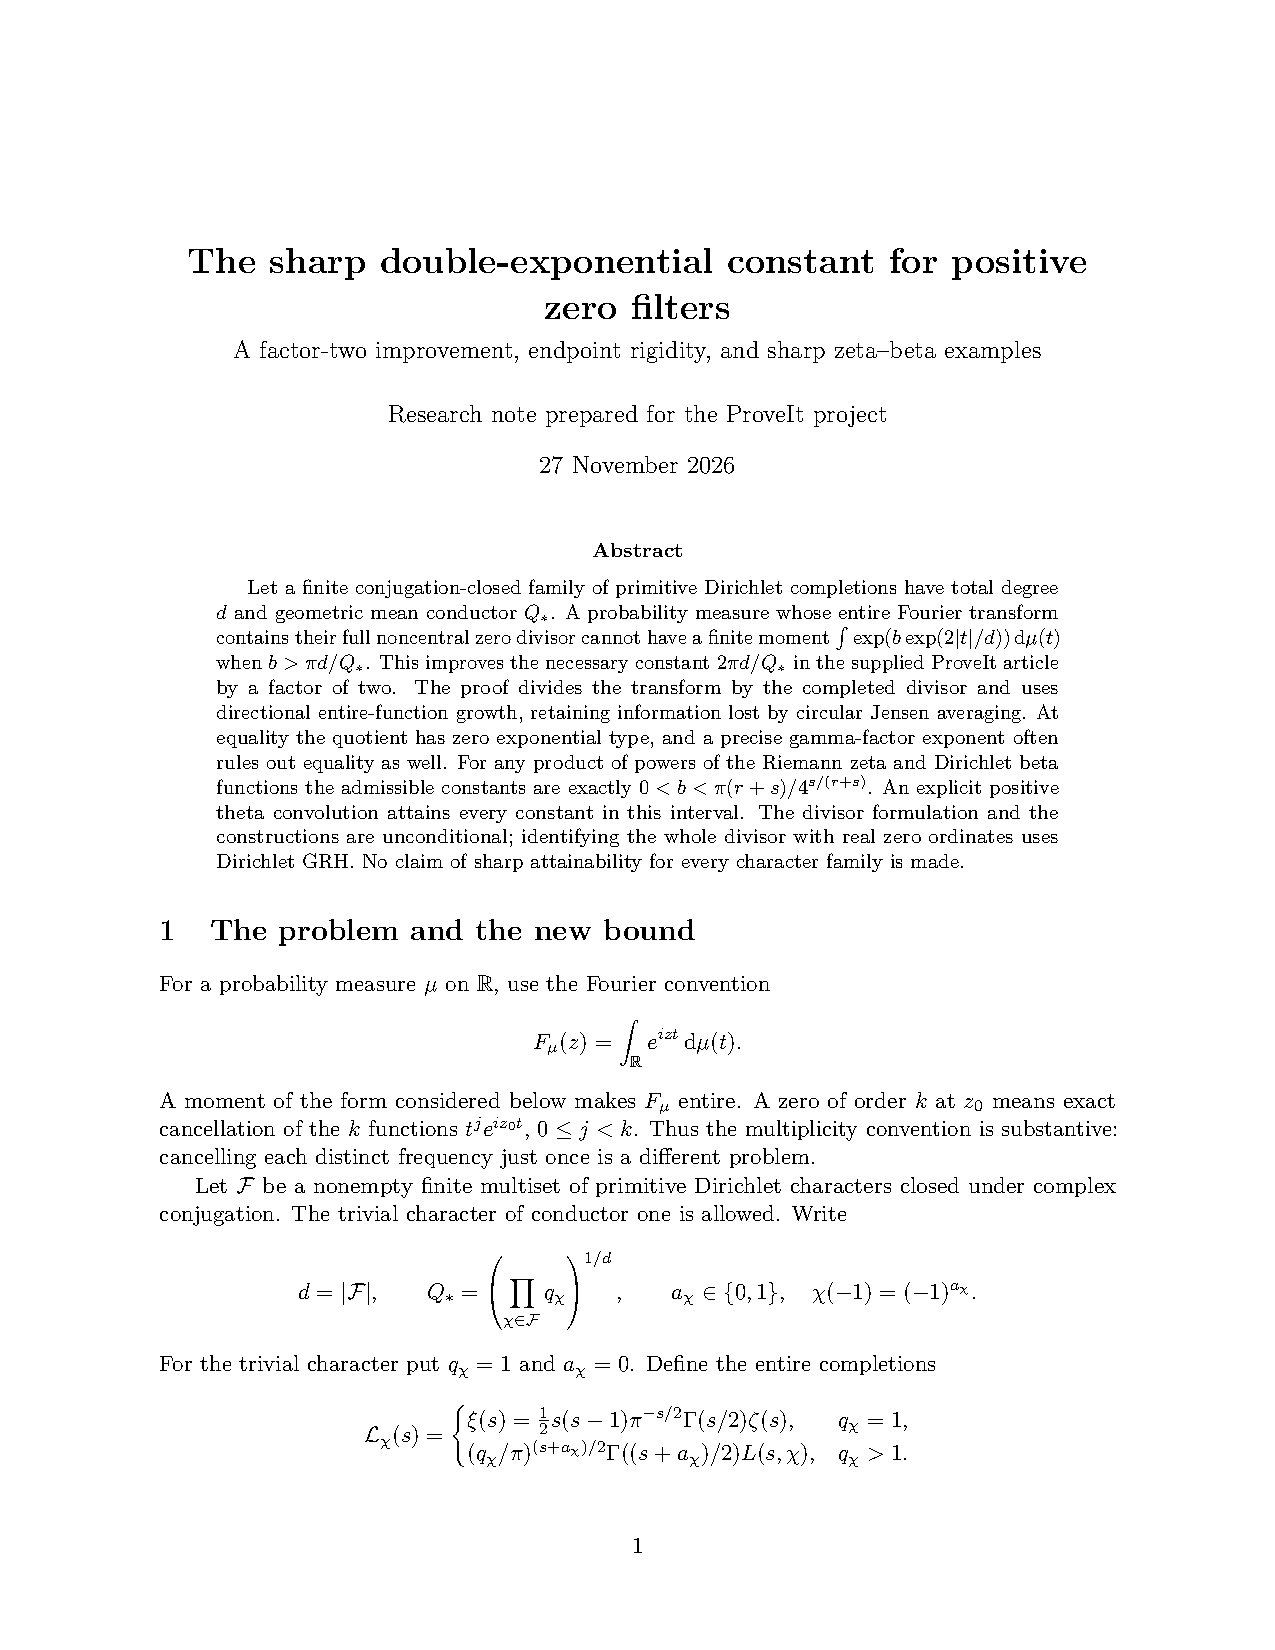
\includepdf[pages=-,fitpaper=true,addtotoc={1,section,1,{Note 1: Sharp endpoint filters},note1}]{01_endpoint_filters/paper.pdf}
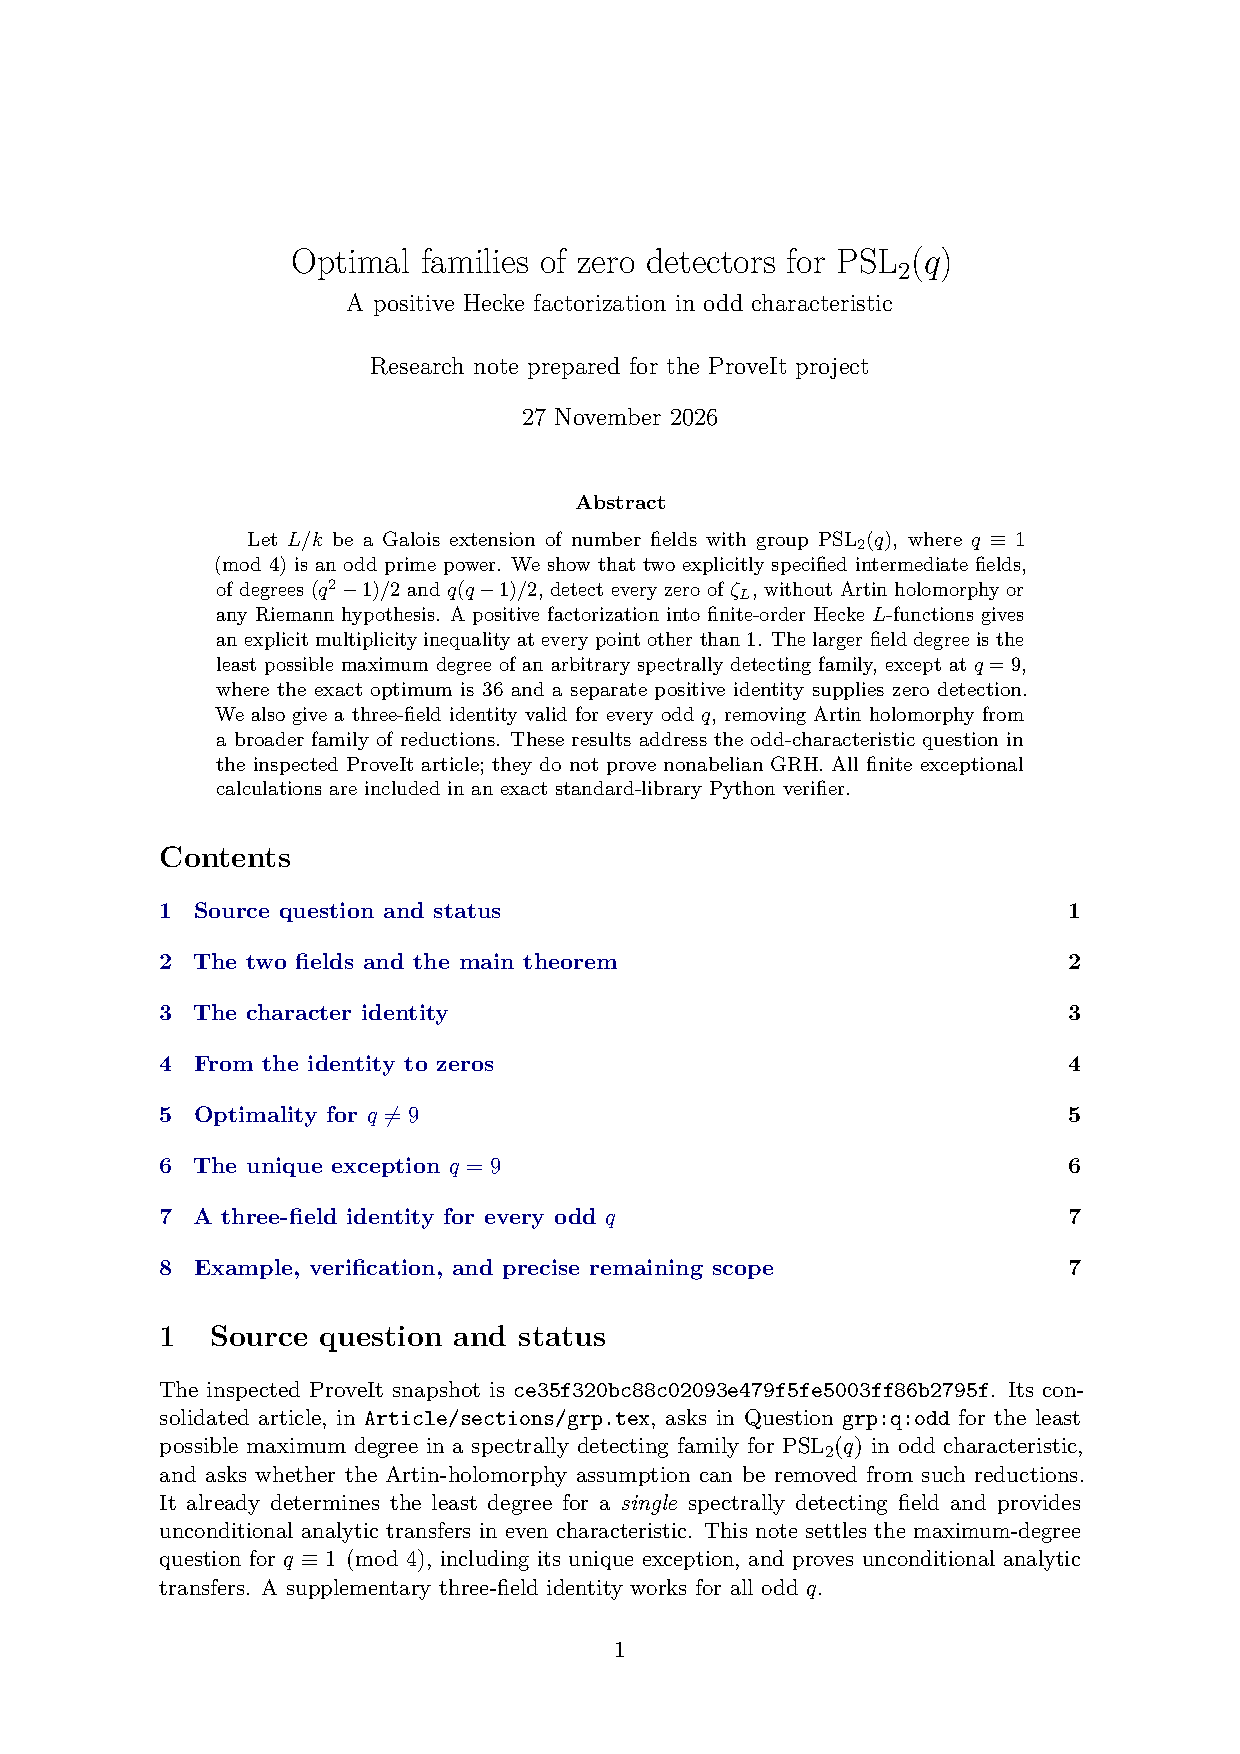
\includepdf[pages=-,fitpaper=true,addtotoc={1,section,1,{Note 2: Optimal PSL2 subfield detectors},note2}]{02_psl2_detectors/psl2_detector.pdf}
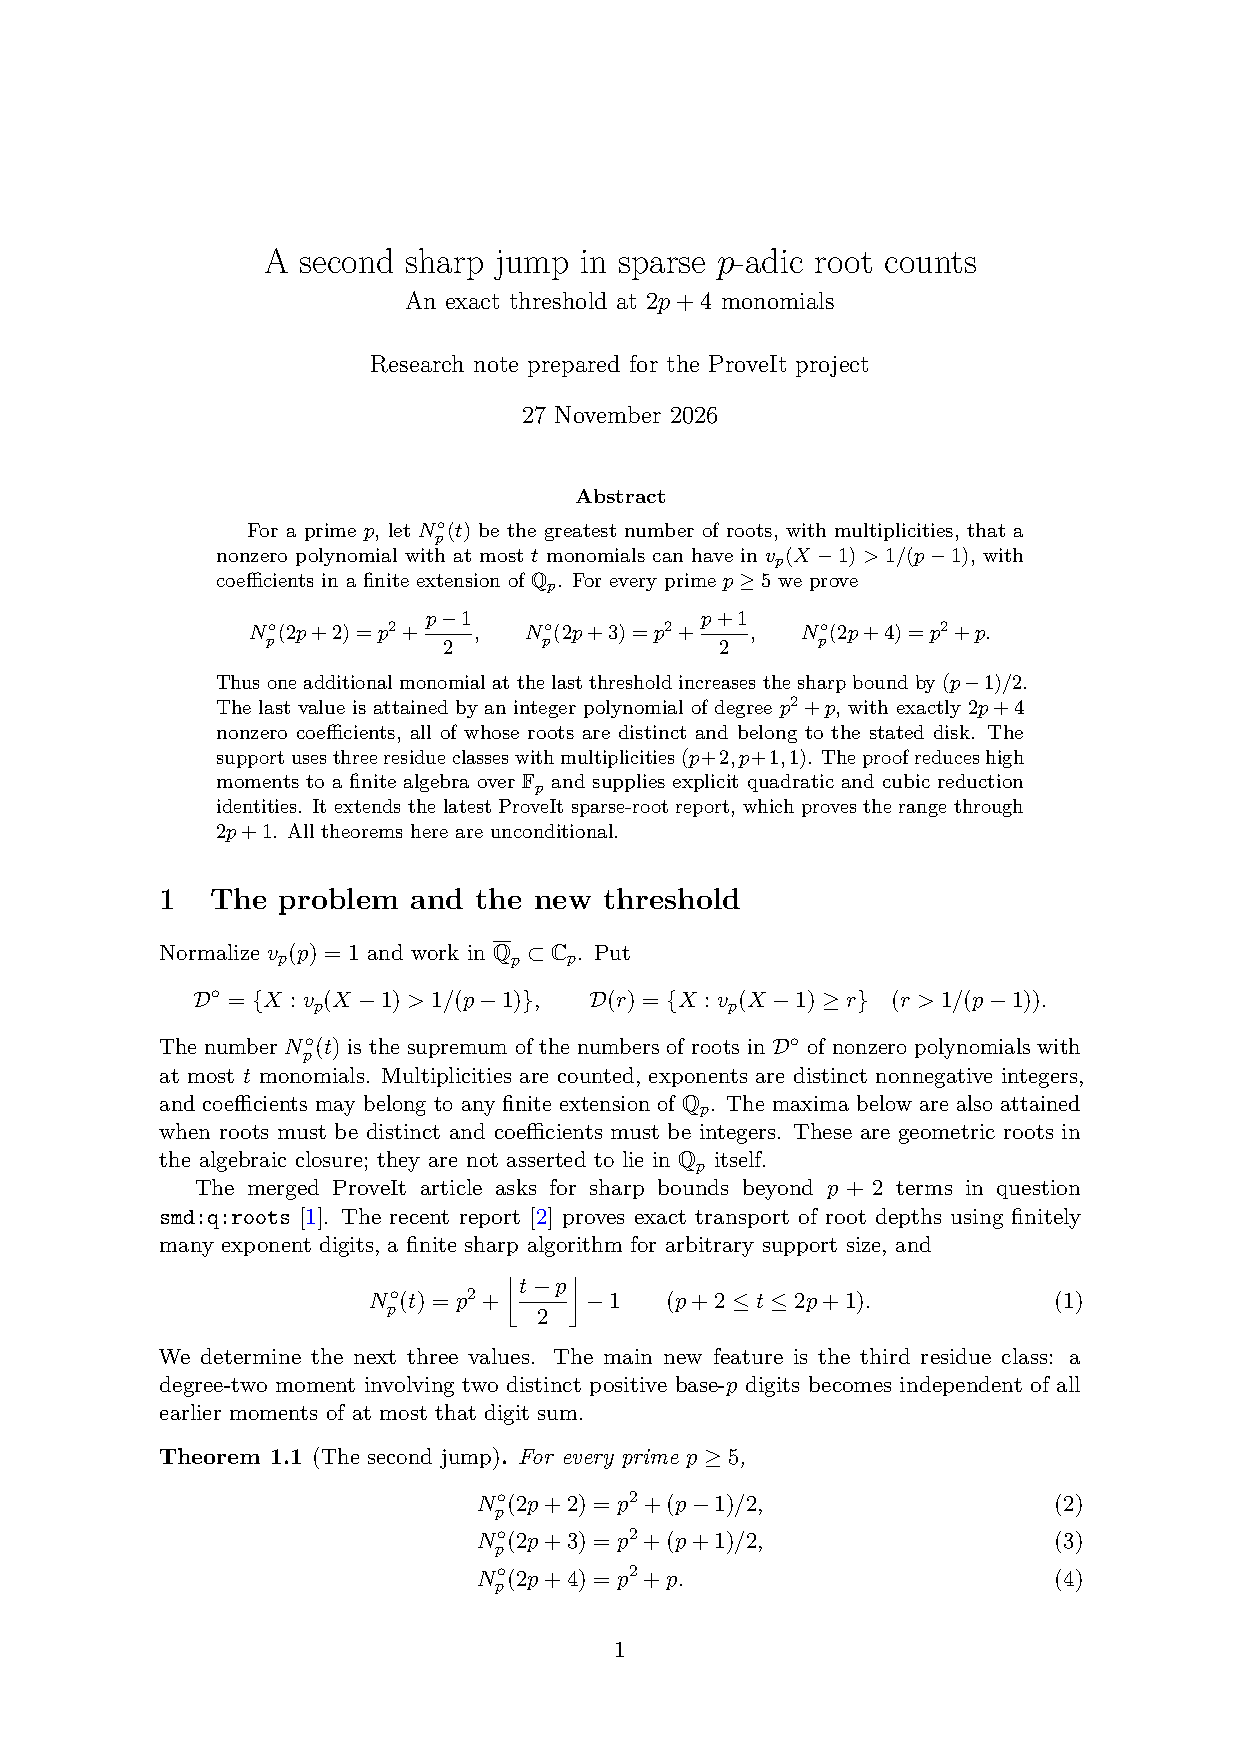
\includepdf[pages=-,fitpaper=true,addtotoc={1,section,1,{Note 3: Sparse p-adic root threshold},note3}]{03_sparse_padic/sparse_padic_jump.pdf}
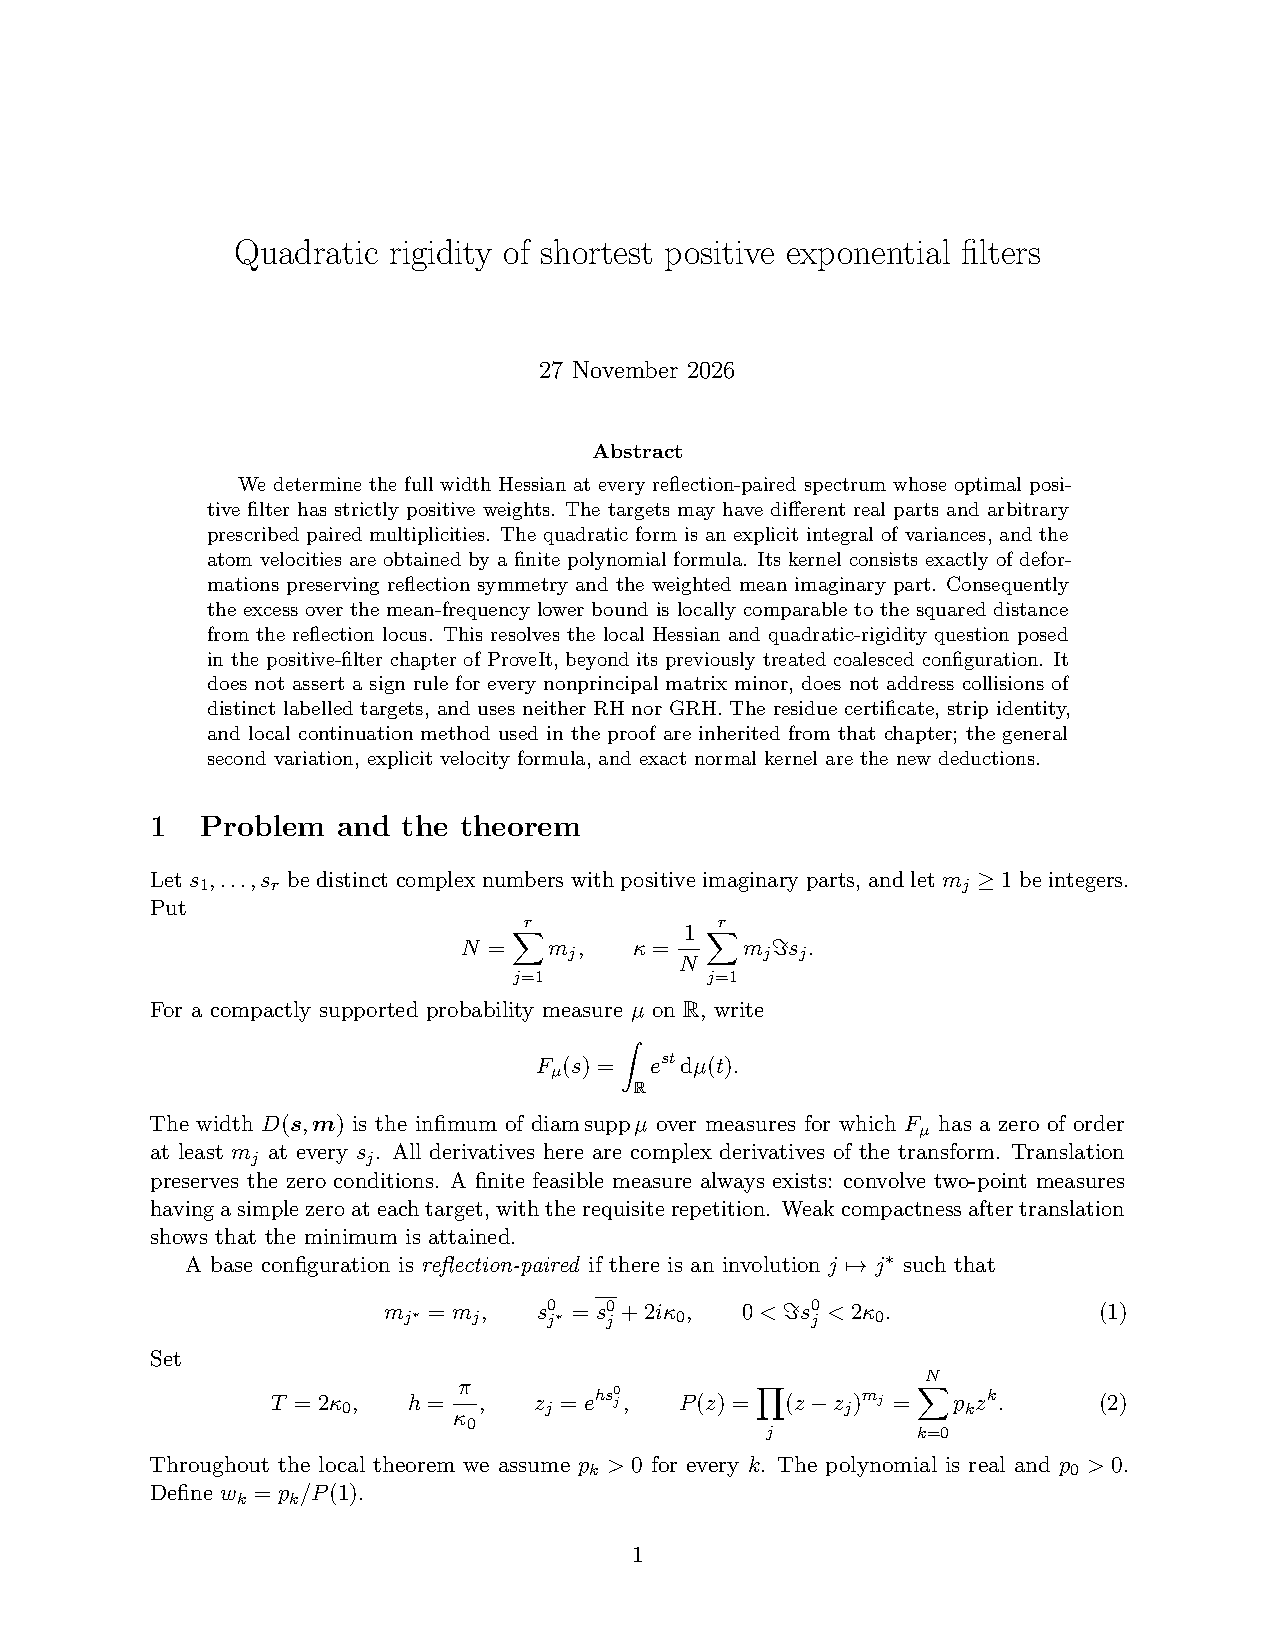
\includepdf[pages=-,fitpaper=true,addtotoc={1,section,1,{Note 4: Quadratic filter rigidity},note4}]{04_mirror_hessian/paper.pdf}
\end{document}
